% Some commands used in this file
The following section covers the theory of kernel methods and introduces the building blocks underlying it.
% \section{Kernel mean embedding of distributions: A review and beyond}

% \href{https://arxiv.org/abs/1605.09522}{
% From this first paper \cite{Muandet_2017}, the notation and terms used in the theory of Reproducing Kernel Hilbert Spaces are summarized.
% \\

Many algorithms use the inner product as similarity measure between the data instances $x, y \in \mathcal{X}$. However, this inner product spans only the class of linear similarity measures. 
\\
The idea behind kernel methods is to apply a non-linear transformation $\phi$ to the data $x$ 
in order to get a more powerful non linear similarity measure.
\begin{align*}
\phi(x)\colon \mathcal{X} &\to \mathcal{H}
    \\
    x&\mapsto \phi(x)
\end{align*}

We take then the inner product in the high dimensional space $\mathcal{H}$ mapped by $\phi(x)$, i.e.\

\begin{align*}
k(x,y):=&\langle \phi(x), \phi(y) \rangle_{\mathcal{H}}
\end{align*}

where $\phi(x)$ is referred to as feature map while $k$ is the kernel function.
Therefore, we can kernelize any algorithm involving a dot product by substituting $\langle x, y \rangle_{\mathcal{X}}$ with $\langle \phi(x), \phi(y) \rangle_{\mathcal{H}}$

One would expect constructing the feature maps explicitly and then evaluating their inner product in $\mathcal{H}$ to be computationally expensive, and indeed it is. However, we do not have to explicitly perform such calculations. This is because of the kernel trick.
To illustrate the idea behind the kernel trick consider the following example.
Suppose $x, y \in \mathbb{R}^2$ and assume $\phi(x)=(x_{1}^{2},x_{2}^{2},\sqrt{2}x_{1}x_{2})$, then the inner product in the feature space is $x_{1}^{2}y_{1}^{2}+x_{2}^{2}y_{2}^{2}+2x_{1}x_{2}y_{1}y_{2}$.
Notice that this is the same of $\langle \phi(x), \phi(y) \rangle_{\mathcal{H}}$; thus the kernel trick consists of just using $k(x,y):=(x^\intercal y)^2$.
For instance:

$$
\begin{aligned}
\langle \phi([2,4]),\phi([8,9]) \rangle_{\mathcal{H}}&=  \left[ {\begin{array}{cccc}
    4 & 16 &     \sqrt{2}\cdot 2 \cdot 4\\
  \end{array} } \right]
  \left[ {\begin{array}{cccc}
    64\\
    81\\
    \sqrt{2}\cdot8 \cdot 9
    \\
  \end{array} } \right]\\ &=4\cdot 64 +16\cdot 81 +2 \cdot 2 \cdot 4 \cdot 8 \cdot 9=2704
\end{aligned}
$$

While $k([2,4], [8,9])=(16+36)^2=2704$
We can see that the latter calculation is much quicker and compact.
This gives a taste of how powerful kernels are thanks to the kernel trick.
Indeed, the idea of the the kernel trick can be extended to feature maps
$\phi$ involving an infinite feature space. In these cases, calculating the
respective kernel is equal to calculating the inner product between an infinite
number of features of the data points.

\section{Theory of kernels}
Subsequently, we introduce the definitions that make up the basis for the theory of kernel methods.

\begin{definition}
    A sequence $\{v_n\}_{n=1}^{\infty}$ of elements of a normed vector space $\mathcal{V}$ is a Cauchy sequence if for every $\epsilon>0$, there exist $N=N(\epsilon) \in \mathbb{N}$ such that $\|v_n-v_m\|_{\mathcal{V}}<\epsilon \ \ \forall m,n\geq N$  
\end{definition}

\begin{definition}
    A sequence $\{v_n\}_{n=1}^{\infty}$ is convergent if for every $\epsilon>0$ there exists $N=N(\epsilon) \in \mathbb{N}$ and a point $ v \in \mathcal{V}$ such that  $\|v_n-v\|_{\mathcal{V}} < \epsilon$ $\forall n\geq N$.
\end{definition}

\begin{definition}
    A complete normed space is a normed vector space in which every Cauchy sequence is convergent.
\end{definition}


\begin{definition}
    A Hilbert space is a vector space $\mathcal{H}$ with an inner product $\langle \cdot, \cdot \rangle_{\mathcal{H}}$ such that the norm defined by $\|f\|_{\mathcal{H}}=\sqrt{\langle f, f \rangle}_{\mathcal{H}}$
turns $\mathcal{H}$ into a complete normed vector space.
\end{definition}




\begin{definition}
    Considering a set of vectors $x_1, \cdots, x_m \in \mathcal{X} \subseteq \mathbb{R}^n$, the Gram matrix is defined as the $n\times n$ matrix whose entries are $\langle x_i, x_j \rangle_{\mathcal{X}}$.    
\end{definition}

It follows from the definition that the Gram matrix is symmetric.
In the kernel setting we evaluate the inner products in the feature space generated by the feature map $\phi$, therefore the Gram matrix will have entries $\langle \phi(x_i), \phi(x_j) \rangle_{\mathcal{H}}= k(x_i, x_j)$. Such matrix is also referred to as the kernel matrix $K$.

\[
K_{m\times m}=
\begin{bmatrix}
    k(x_1,x_1)       &  \dots & k(x_1,x_n) \\
    \vdots       & \ddots & \vdots \\
    k(x_n, x_1)       & \dots & k(x_n, x_n)
\end{bmatrix}
\]
% All kernel methods take as input the kernel matrix, it is the central data type for all 
% such techniques.

\begin{proposition}
    In addition to being symmetric, $K$ possesses also the property of being positive semidefinite.    
\end{proposition}

\begin{proof}
    $$
    \begin{aligned}
        z^\intercal K z =& \sum_{i,j=1}^n z_i z_j k(x_i,x_j)
        \\
        =& \sum_{i,j=1}^n z_i z_j \langle \phi(x_i), \phi(x_j) \rangle_{\mathcal{H}}
        \\
        =& \left\langle \sum_{i=1}^n z_i \phi(x_i), \sum_{j=1}^n z_j \phi(x_j)\right\rangle_{\mathcal{H}}
        \\
        =& \left\|\sum_{i=1}^n z_i \phi(x_i) \right\|_{\mathcal{H}}^2 \geq 0
    \end{aligned}
    $$
\end{proof}
We know that positive semidefinite matrices form a cone in the vector space of $n\times n$ matrices. Because of this, we have that the set of such matrices is convex, this implies that the theory of convex analysis can be used when optimising over them.


\begin{definition}
    A function $k: \mathcal{X} \times \mathcal{X} \to \mathbb{R}$ is said to be finitely positive semidefinite if it is a symmetric function for which the matrices formed by restriction to any finite subset of the space $\mathcal{X}$ are positive semidefinite.
\end{definition}

\begin{theorem}[Characterisation of kernels \cite{shawe2004kernel}]    
    A function $k:\mathcal{X} \times \mathcal{X} \to \mathbb{R}$ which is either continous or has finite domain can be decomposed as $k(x,y)=\langle \phi(x), \phi(y) \rangle_{\mathcal{H}}$ if and only if $k$ is positive semidefinite.
\end{theorem}

The theorem implies that the function $k$ can be written as the inner product in the Hilbert space $\mathcal{H}$ of the features evaluated at the arguments $\phi(x)$.

Next, we make this characterisation explicit by showing how to construct a feature mapping $\phi$ of a kernel $k$ such that it is positive semidefinite.
Let the feature space be the set of functions 

$$ 
\begin{aligned}
    \mathcal{F} =\bigg\{ \sum\limits_{i=1}^n \alpha_i k(x_i, \cdot): n \in \mathbb{N}, x_i, y_i \in \mathcal{X}, a_i \in \mathbb{R}, i=1,\cdots, n \bigg\}    
\end{aligned}
$$
This space is clearly closed under addition of functions and scalar multiplication. Therefore, it is a vector space.
Letting $f(x)=\sum\limits_{i=1}^n \alpha_i k_i(x_i,x)$ and $g(x)=\sum\limits_{i=1}^m \beta_i k_i(y_i,x)$,  we can introduce an inner product on $\mathcal{F}$ as 

$$
\begin{aligned}
    \langle f,g \rangle_{\mathcal{F}}:=\sum\limits_{i=1}^n\sum\limits_{j=1}^m a_i \beta_j k_i(x_i,y_j)=\sum\limits_{i=1}^n a_i g(x_i)= \sum\limits_{j=1}^m \beta_j f(y_j)
\end{aligned}
$$

Notice, $\langle f, f \rangle_{\mathcal{F}}= \alpha^\intercal K \alpha \geq 0 \ \forall f \in \mathcal{F}$, where $K$ is the kernel matrix.
Moreover, $\langle f, g \rangle_{\mathcal{F}}$ is real valued, symmetric and bilinear and, hence, an inner product.

Additionally, letting $g(x)=k(\cdot, x)$, we have that 
\begin{equation}
    \langle f, k(\cdot, x)\rangle_{\mathcal{F}}=\sum\limits_{i=1}^n a_i k(x_i,x)=f(x)    
\end{equation}
This is known as the reproducing property.

Finally, we extend $\mathcal{F}$ to a complete vector space.
Consider a fixed input $x$ and a Cauchy sequence $\{f_n\}_{n=1}^{\infty}$, we then have by means of the Cauchy-Schwarz inequality that 

\begin{equation}
    (f_n(x)- f_m(x))^2=\langle f_n-f_m, k(\cdot, x)\rangle_{\mathcal{F}}^2 \leq \| f_n - f_m \|_{\mathcal{F}}^2 k(x,x)    
\end{equation}

We have then, that $f_n(x)$ is a Cauchy sequence of real numbers. Thus, we can let $g(x):=\underset{n\to \infty}\lim f_n(x)$ and add all such limits functions to $\mathcal{F}$, doing so we complete $\mathcal{F}$ and we obtain the Hilbert space $\mathcal{H}$ associated to the kernel $k$.
Having constructed the feature space $\mathcal{H}$, the mapping $\phi(x)$ is defined as

\begin{equation}
    \phi: x \in \mathcal{X} \to \phi(x)=k(\cdot, x) \in \mathcal{H}
\end{equation}

Notice, that by the reproducing property, $f$ can be represented as the inner product with itself in the feature space, that is 
\begin{equation}
    f(x)=\langle f, \phi(x)\rangle_{\mathcal{H}}=\langle f, k(\cdot, x)\rangle_{\mathcal{H}}=f(x)
\end{equation}

\begin{definition}
    Let $(\mathcal{H}, \langle \cdot, \cdot \rangle_\mathcal{H})$ be a Hilbert space of real-valued functions on $\mathcal{X}$. A function $k: \mathcal{X} \times \mathcal{X} \to \mathbb{R}$ is called a reproducing kernel of $\mathcal{H}$ if and only if 
     \begin{align}
        k(x, \cdot) \in \mathcal{H} &\quad \ \forall x \in \mathcal{X}    \\
        \langle  f, k(x, \cdot) \rangle_\mathcal{H} = f(x) &\quad \ \forall f\in \mathcal{H}, \ x \in \mathcal{X}
    \end{align}
    Notice, positive semidefiniteness property of kernel $k$ is a sufficient condition for $\mathcal{H}$ to have an associated RKHS.
\end{definition}

The analysis above applies to any kernel, that is, given a valid kernel function we can always construct its RKHS in the way we just illustrated.
\begin{theorem}
    If a symmetric function $k(\cdot, \cdot)$ satisfies the reproducing property in a Hilbert space $\mathcal{H}$, then $k$ is positive semidefinite.
\end{theorem}

\begin{proof}
    \begin{align}
        \sum\limits_{i,j=1}^n a_i a_j k(x_i, x_j)=& \sum\limits_{i,j=1}^n a_i a_j \langle k(\cdot, x_i), k(\cdot, x_j)\rangle_{\mathcal{H}}
        \\
        =& \left\langle \sum\limits_{i=1}^n a_i k(\cdot, x_i), \sum\limits_{j=1}^n a_j k(\cdot, x_j) \right\rangle_{\mathcal{H}} \\
        =& \left\| \sum\limits_{i=1}^n a_i k(x_i, x_i)\right\|_{\mathcal{H}}^2 \geq 0
    \end{align}
\end{proof}
   
% \begin{definition}
%     RKHS.
%     A Reproducing Kernel Hilbert Space is a Hilbert space with the evaluation functionals $\mathcal{F}_{x}(f):=f(x)$ bounded, i.e. $\forall x \in \mathcal{X}$ there exists some $C>0$ such that $\| \mathcal{F}_{x}(f)\|=\|f(x)\| \leq C \|f\|_{\mathcal{H}} \ \forall f \in \mathcal{H}$
% \end{definition}


\begin{theorem}
    [Riesz Representation \cite{Conway1994-kh}] If $L : \mathcal{H} \rightarrow \mathbb{R}$ is a bounded linear operator on a Hilbert space $\mathcal{H}$ , there exists some $h_0 \in \mathcal{H}$ such that $L(f) = \langle f,h_0\rangle_\mathcal{H}, \ \forall f \in \mathcal{H}$.
\end{theorem}

% \begin{proof}
%     It is known that the null space of $L$, call it $M$, is a closed linear subspace in $\mathcal{H}$. This implies that the Hilbert space direct sum $M \bigoplus M^\bot$ is an isomorphism of $\mathcal{H}$. When $L(f) \neq 0$ we have that $L(f)=L(m +w)$ with $m \in M$ and $w \in M^\bot$, it follows that $L(f)=0+L(w) \neq 0 \implies$ $M^\bot \neq {0}$.
%     \\
%     Using this fact, we can now choose a $z \in M^\bot$ with norm 1. By linearity of $L$, for any $f \in \mathcal{H}$ we have $L(zL(f)- fL(z))=L(z)L(f)- L(f)L(z)=0$. This means that $zL(f)- fL(z)$ belongs to the null space of $L$, that is  $zL(f)- fL(z) \in M$. 
%     \\
%     Consider now 
%     \begin{align}
%         L(f)=& L(f) \cdot 1
%         \\
%         =& L(f) \langle z,z\rangle_{\mathcal{H}}
%         \\
%         =& \langle zL(f), z\rangle_{\mathcal{H}} \\
%         =& \langle zL(f) -fL(z)+fL(z), z\rangle_\mathcal{H}
%         \\
%         =& \langle zL(f) -fL(z), z\rangle_{\mathcal{H}}+\langle fL(z), z\rangle_{\mathcal{H}} \\
%         % this is zero zL(f) -fL(z), so
%         =& \langle fL(z), z\rangle_{\mathcal{H}} \\
%         =& \langle f, z\overline{L(f)}\rangle_{\mathcal{H}} \\
%     \end{align}
%     Therefore, $L(f)=\langle f, h_0\rangle$  with  $h_0=z\overline{L(z)}$
%     \\
%     Finally, notice that $h_0$ is unique.
%     Assuming $h_0$ and $h_1$ to both satisfy the above equation for all $f \in \mathcal{H}$ we have that
%     \begin{align}
%         \langle h_0,f \rangle_{\mathcal{H}}=&\langle h_1, f \rangle_{\mathcal{H}} \\
%         \langle h_0,f \rangle_{\mathcal{H}}-\langle h_1, f \rangle_{\mathcal{H}}=& 0 \\
%         \langle h_0 -h_1,f \rangle_{\mathcal{H}}=& 0
%     \end{align}
%     Setting $f=h_0 -h_1$, we have the uniqueness of $h_0$.
%     % because inner product is zero, inner product has to satisfy positive definitness property to be such >=0, if it is zero it means that its argument x in <x,x> is zero => h_0=h_1
    
% \end{proof}

%conjugate simmetry is because in complex analysis when you swap in the inner product, you have to take the conjugate


The Riesz representation theorem results in the following proposition for reproducing kernel Hilbert spaces.
\begin{proposition}
For each $x \in \mathcal{X}$ there exists a function $k(\cdot, x) \in \mathcal{H}$ such that the evaluation functional $F_{x}(f)=\langle k(\cdot, x), f\rangle_{\mathcal{H}}=f(x)$    
\end{proposition}

The function $k(\cdot, x)$ is the reproducing kernel evaluated at point $x$.
Furthermore, note that $k(\cdot, x)$ is itself a function lying in it
\begin{align*}
    k(y, x)=F_{y}(k(\cdot, x))=\langle k(\cdot, x), k(\cdot, y)\rangle_{\mathcal{H}}=\langle \phi(x), \phi(y)\rangle_{\mathcal{H}}
\end{align*}


% Kernel functions are characterised by a couple of properties that make them a closure. Thus, there exists ways of combining known kernels in order to obtain new kernels.

\begin{proposition}
    Let $k_1$ and $k_2$ be kernels over $\mathcal{X} \times \mathcal{X}, \mathcal{X} \subseteq \mathbb{R}^n$, $a \in \mathbb{R}^+$ and $\phi: \mathcal{X} \to \mathbb{R}^N$ with $k_3$ a kernel over $\mathbb{R}^N \times \mathbb{R}^N$. Then the following functions are valid kernels:
    $$
    \begin{aligned}
        k(x,y)=&k_1(x,y)+k_2(x,y)
        \\
        k(x,y)=& ak_1(x,y)
        \\
        k(x,y)=& k_1(x,y)k_2(x,y)
        \\
        k(x,y)=& k_3(\phi(x),\phi(y))
    \end{aligned}
    $$.
\end{proposition}

\begin{proof}
    Consider a finite set of points $x_1, \cdots, x_n$, a vector $z \in \mathbb{R}^n$ and let $K_1$ and $K_2$ be the kernel matrices associated to $k_1$ and $k_2$ evaluated on these points.

    We have:

    $$  
    \begin{aligned}
    z^\intercal (K_1+K_2) z&= z^\intercal K_1 z + z^\intercal K_2 z \geq 0
    \\
    z^\intercal aK z&= a z^\intercal K z \geq 0
    \end{aligned}
    $$
    Let $K=K_1 \otimes K_2$, we have that the eigenvalues of $K$ are made up by the product pairs of the eigenvalues of $K_1$ and $K_2$. Thus, $K$ is positive semidefinite. Next, the matrix given by $k_1 \cdot k_2$ corresponds to the Schur product of $K_1$ and $K_2$, denote it $H$. Notice, $H$ is a principal submatrix of $K$, hence for any $z \in \mathbb{R}^n$ there exist a $t \in \mathbb{R}^{n^2}$ such that $z^\intercal H z= t^\intercal K t$. Using the fact that K is positive semidefinite we have that for any $z$, it holds 
    $$
    \begin{aligned}
        z^\intercal H z= t^\intercal K t\geq 0
    \end{aligned}
    $$
\end{proof}

\section{Kernel families}\label{kernel families}
The selection of the kernel determines the class of functions that will be searched by the learning algorithm. Prior knowledge of the problem domain can help restricting the candidate families of kernel functions.
Table \ref{tab:kernel types} contains popular kernel families in literature and applications.
\begin{table}
    \caption{Kernel types}
    \resizebox{\textwidth}{!}{
    \begin{tabular}{lll}
        \toprule
       Kernel function & Equation & Hyperparameters \\
       \midrule
       Linear &  $k(x,y)=x^\intercal y$ &   \\
       Polynomial &  $k(x,y)=(x^\intercal y+c)^d$ &   c, d\\
       Gaussian RBF &  $k(x,y)=\exp\left(-\frac{\|x-y\|_{2}^2}{2 l^2}\right)$ &   $l$\\
       Exponential RBF/Laplacian& $k(x,y)=\exp\left(-\frac{\|x-y\|_{2}}{l}\right)$ &   $l$\\
       Absolute Laplacian& $k(x,y)=\exp\left(-\frac{\|x-y\|_{1}}{l}\right)$ &   $l$\\
       Hyperbolic/Sigmoid Kernel &  $k(x,y2)=\tanh(\gamma x^\intercal y+r)$ &  $\gamma$, r \\
       Periodic &  $k(x,y)=\exp\left(\frac{-2 sin^2\left(\frac{\pi}{p}\|x-y\|_{2} \right)}{l^2}\right) $ &   $p, l$\\
       Chi-squared kernel &  $k(x,y)=\exp\left(-\gamma \sum\limits_i \frac{(x_i - y_i)^2}{x_i+y_i}\right) $ &   $\gamma$\\
        Cosine  &  $k(x,y)=\frac{x^\intercal y}{\|x\|_{2}\|y\|_{2}}$ &   \\
       Matern  &  $k(x, y) =  \frac{1}{\Gamma(\nu)2^{\nu-1}}\Bigg(
        \frac{\sqrt{2\nu}}{l} \|x-y|\|_{2}
        \Bigg)^\nu Y_\nu\Bigg(
        \frac{\sqrt{2\nu}}{l} \|x-y|\|_{2}\Bigg)$ &  $l, \nu$ \\

        \bottomrule
    \end{tabular}}
    \label{tab:kernel types}
\end{table}

Notice, in the Matern family, $\Gamma(\cdot)$ is the gamma function while $Y(\cdot)$ is the Bessel function of the second kind.
When $\nu=p+\frac{1}{2}$, $p \in \mathbb{N}$, the Matern kernel can be rewritten as a product of an exponential and a polynomial of degree $p$. 

\begin{equation*}
    \begin{split}
    k(x,y)&=\exp \left(-{\frac {{\sqrt {2p+1}}\|x-y|\|_{2}}{l }}\right){\frac {p!}{(2p)!}}\\
    & \ \cdot \sum\limits_{i=0}^{p}{\frac {(p+i)!}{i!(p-i)!}}\left({\frac {2{\sqrt {2p+1}}\|x-y|\|_{2}}{l }}\right)^{p-i}
\end{split}
\end{equation*}

For example:
\begin{itemize}
    \item $p=0,\nu=\frac{1}{2} \implies k(x,y)=\exp\left(-\frac{\|x-y\|_{2}}{l}\right)$
    \item $p=1,\nu=\frac{3}{2} \implies 
    k(x,y)=\left(1+{\frac {{\sqrt {3}}\|x-y\|_{2}}{l }}\right)\exp \left(-{\frac {{\sqrt {3}}\|x-y\|_{2}}{l }}\right)$
    \item $p=2,\nu=\frac{5}{2} \implies k(x,y)=\left(1+{\frac {{\sqrt {5}}\|x-y\|_{2}}{l }}+{\frac {5\|x-y\|_{2}^{2}}{3 l ^{2}}}\right)\exp \left(-{\frac {{\sqrt {5}}\|x-y\|_{2}}{l }}\right)$
\end{itemize}

When $\nu=\frac{1}{2}$ the Matern kernel corresponds to the Laplacian kernel. If the predictors are one dimensional, then the Absolute Laplacian and the Matern 0.5 are equivalent. %L2 norm=L1 norm
Furthermore, as $\nu \to \infty$ we have that the Matern kernel converges to the Gaussian RBF kernel.
$k(x,y)=\exp\left(\frac{-\|x-y\|_{2}^2}{2l^2}\right)$


% CONDITIONS upon matern is equivalent to rbf
% KERNEL THEORY FROM BOOKS AND KERNEL COOKBOOK


% Any algorithm involving inner products between inputs can be combined with a kernel method. The chosen kernel function will calculate the inner product between the images of two inputs in the feature space. This makes the orginal algorithm operate in a high dimesional space. 
Kernel methods show good modularity because they work the same for any kernel and any data type. This concept is illustrated in Figure \ref{fig:workflow_kernels}, where an abstract kernel methods workflow is visualized. First we build the kernel matrix by using a kernel function to process the input data. Next, the kernel matrix is passed to the pattern analysis (PA) algorithm, which returns the learned function.

\begin{figure}[!ht]
    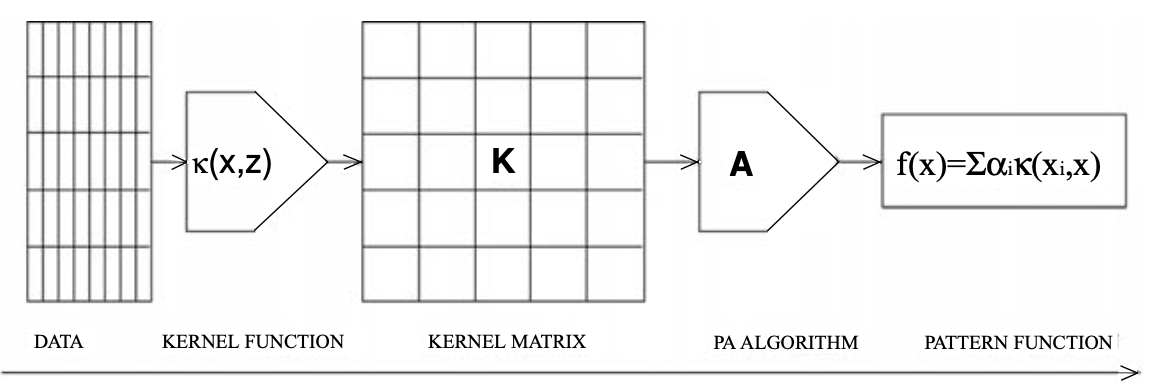
\includegraphics[width=\textwidth]{images/workflow_kernels.png}
    \caption{Workflow for the application of kernel methods \cite{shawe2004kernel}}
    \label{fig:workflow_kernels}
\end{figure}